% !TEX TS-program = XeLaTeX
% use the following command: 
% all document files must be coded in UTF-8
\documentclass{textolivre}
% for anonymous submission
%\documentclass[anonymous]{textolivre}
% to create HTML use 
%\documentclass{textolivre-html}
% See more information on the repository: https://github.com/leolca/textolivre

% Metadata
\begin{filecontents*}[overwrite]{article.xmpdata}
    \Title{Obsolescencia del conocimiento vs formación para el desarrollo sostenible: voces de protagonistas en el marco de la COVID 19}
    \Author{Maria Soledad Ramírez-Montoya}
    \Language{es}
    \Keywords{conocimiento \sep innovación educativa \sep tecnologías \sep educación superior \sep COVID 19}
    \Journaltitle{Texto Livre}
    \Journalnumber{1983-3652}
    \Volume{14}
    \Issue{2}
    \Firstpage{1}
    \Lastpage{16}
    \Doi{10.35699/1983-3652.2021.33840}

    \setRGBcolorprofile{sRGB_IEC61966-2-1_black_scaled.icc}
            {sRGB_IEC61966-2-1_black_scaled}
            {sRGB IEC61966 v2.1 with black scaling}
            {http://www.color.org}
\end{filecontents*}

% used to create dummy text for the template file
\definecolor{dark-gray}{gray}{0.35} % color used to display dummy texts
\usepackage{lipsum}
\SetLipsumParListSurrounders{\colorlet{oldcolor}{.}\color{dark-gray}}{\color{oldcolor}}

% used here only to provide the XeLaTeX and BibTeX logos
\usepackage{hologo}

% used in this example to provide source code environment
%\crefname{lstlisting}{lista}{listas}
%\Crefname{lstlisting}{Lista}{Listas}
%\usepackage{listings}
%\renewcommand\lstlistingname{Lista}
%\lstset{language=bash,
        breaklines=true,
        basicstyle=\linespread{1}\small\ttfamily,
        numbers=none,xleftmargin=0.5cm,
        frame=none,
        framexleftmargin=0.5em,
        framexrightmargin=0.5em,
        showstringspaces=false,
        upquote=true,
        commentstyle=\color{gray},
        literate=%
           {á}{{\'a}}1 {é}{{\'e}}1 {í}{{\'i}}1 {ó}{{\'o}}1 {ú}{{\'u}}1 
           {à}{{\`a}}1 {è}{{\`e}}1 {ì}{{\`i}}1 {ò}{{\`o}}1 {ù}{{\`u}}1
           {ã}{{\~a}}1 {ẽ}{{\~e}}1 {ĩ}{{\~i}}1 {õ}{{\~o}}1 {ũ}{{\~u}}1
           {â}{{\^a}}1 {ê}{{\^e}}1 {î}{{\^i}}1 {ô}{{\^o}}1 {û}{{\^u}}1
           {ä}{{\"a}}1 {ë}{{\"e}}1 {ï}{{\"i}}1 {ö}{{\"o}}1 {ü}{{\"u}}1
           {Á}{{\'A}}1 {É}{{\'E}}1 {Í}{{\'I}}1 {Ó}{{\'O}}1 {Ú}{{\'U}}1
           {À}{{\`A}}1 {È}{{\`E}}1 {Ì}{{\`I}}1 {Ò}{{\`O}}1 {Ù}{{\`U}}1
           {Ã}{{\~A}}1 {Ẽ}{{\~E}}1 {Ũ}{{\~u}}1 {Õ}{{\~O}}1 {Ũ}{{\~U}}1
           {Â}{{\^A}}1 {Ê}{{\^E}}1 {Î}{{\^I}}1 {Ô}{{\^O}}1 {Û}{{\^U}}1
           {Ä}{{\"A}}1 {Ë}{{\"E}}1 {Ï}{{\"I}}1 {Ö}{{\"O}}1 {Ü}{{\"U}}1
           {ç}{{\c{c}}}1 {Ç}{{\c{C}}}1
}


\journalname{Texto Livre}
\thevolume{14}
\thenumber{2}
\theyear{2021}
\receiveddate{\DTMdisplaydate{2020}{12}{11}{-1}} % YYYY MM DD
\accepteddate{\DTMdisplaydate{2021}{2}{28}{-1}}
\publisheddate{\today}
% Corresponding author
\corrauthor{Maria Soledad Ramírez-Montoya}
% DOI
\articledoi{10.35699/1983-3652.2021.33840}
% list of available sesscions in the journal: articles, dossier, reports, essays, reviews, interviews, editorial
\articlesessionname{dossier}
% Abbreviated author list for the running footer
\runningauthor{Ramírez-Montoya}
\editorname{Daniervelin Pereira}

\title{Obsolescencia del conocimiento vs formación para el desarrollo sostenible: voces de protagonistas en el marco de la COVID 19}
\othertitle{Obsolescência do conhecimento e formação para o desenvolvimento sustentável: vozes dos protagonistas no âmbito da COVID 19}
\othertitle{Obsolescence of knowledge vs. training for sustainable development: voices of protagonists in the framework of COVID 19}
% if there is a third language title, add here:
%\othertitle{Artikelvorlage zur Einreichung beim Texto Livre Journal}

\author[1]{Maria Soledad Ramírez-Montoya \orcid{0000-0002-1274-706X} \thanks{Email: \url{solramirez@tec.mx}}}

\affil[1]{Tecnologico de Monterrey, Escuela de Humanidades y Educación, Departamento de Educación, Monterrey, México.}

\addbibresource{article.bib}
% use biber instead of bibtex
% $ biber tl-article-template

% set language of the article
\setdefaultlanguage{spanish}
\setotherlanguage{portuguese}
\setotherlanguage{english}

% for spanish, use:
%\setdefaultlanguage{spanish}
%\gappto\captionsspanish{\renewcommand{\tablename}{Tabla}} % use 'Tabla' instead of 'Cuadro'
%\AfterEndPreamble{\crefname{table}{tabla}{tablas}\Crefname{table}{Tabla}{Tablas}}

% for languages that use special fonts, you must provide the typeface that will be used
% \setotherlanguage{arabic}
% \newfontfamily\arabicfont[Script=Arabic]{Amiri}
% \newfontfamily\arabicfontsf[Script=Arabic]{Amiri}
% \newfontfamily\arabicfonttt[Script=Arabic]{Amiri}
%
% in the article, to add arabic text use: \textlang{arabic}{ ... }

% to use emoticons in your manuscript
% https://stackoverflow.com/questions/190145/how-to-insert-emoticons-in-latex/57076064
% using font Symbola, which has full support
% the font may be downloaded at:
% https://dn-works.com/ufas/
% add to preamble:
% \newfontfamily\Symbola{Symbola}
% in the text use:
% {\Symbola }

% reference itens in a descriptive list using their labels instead of numbers
% insert the code below in the preambule:
\makeatletter
\let\orgdescriptionlabel\descriptionlabel
\renewcommand*{\descriptionlabel}[1]{%
  \let\orglabel\label
  \let\label\@gobble
  \phantomsection
  \edef\@currentlabel{#1\unskip}%
  \let\label\orglabel
  \orgdescriptionlabel{#1}%
}
\makeatother
%
% in your document, use as illustraded here:
%\begin{description}
%  \item[first\label{itm1}] this is only an example;
%  % ...  add more items
%\end{description}
 

% custom epigraph - BEGIN 
%%% https://tex.stackexchange.com/questions/193178/specific-epigraph-style
\usepackage{epigraph}
\renewcommand\textflush{flushright}
\makeatletter
\newlength\epitextskip
\pretocmd{\@epitext}{\em}{}{}
\apptocmd{\@epitext}{\em}{}{}
\patchcmd{\epigraph}{\@epitext{#1}\\}{\@epitext{#1}\\[\epitextskip]}{}{}
\makeatother
\setlength\epigraphrule{0pt}
\setlength\epitextskip{0.5ex}
\setlength\epigraphwidth{.7\textwidth}
% custom epigraph - END


% if you use multirows in a table, include the multirow package
\usepackage{multirow}

% add line numbers for submission
%\usepackage{lineno}
%\linenumbers

\begin{document}
\maketitle

\begin{polyabstract}
\begin{abstract}
A lo largo de la historia se ha demostrado que el conocimiento ha sido un bien preciado para el crecimiento personal, profesional y para el desarrollo científico y social. En época de crisis, como la COVID 19, estos bienes reflejan un motor para el desarrollo sostenible. El objetivo del presente artículo es aportar datos de estudiantes y egresados que cursan y han cursado posgrados de Humanidades y Educación, en ambientes presenciales y a distancia, que den cuenta de sus motivaciones, los conocimientos y las competencias necesarias que les permitan ser actores protagónicos y ser generadores de los cambios en la sociedad. El artículo se focalizó en la aplicación de diversos instrumentos para obtener “las voces” de 454 estudiantes y egresados, con cuestionarios que recogieron las motivaciones y percepciones que los encuestados tenían de los programas. Los datos dieron cuenta que se requieren conocimientos que atiendan las dinámicas de las problemáticas y transformaciones de los ambientes de trabajo, así como el desarrollo de competencias relacionadas con la investigación, la innovación y las tecnologías. Se concluye que, en la formación, se hace imprescindible la vinculación constante con diversos sectores de la sociedad, en un trabajo multidisciplinar, interinstitucional y solidario. Este estudio puede ser de valor para profesores, investigadores, diseñadores, emprendedores, tecnólogos, directivos y tomadores de decisiones, interesados en promover ambientes formativos que apoyen el desarrollo sostenible de capacidades científicas, tecnológicas y de innovación que posibiliten un impacto en las transformaciones sociales.

\keywords{Conocimiento \sep Innovación educativa \sep Tecnologías \sep Educación superior \sep COVID 19}
\end{abstract}

\begin{portuguese}
\begin{abstract}
Ao longo da história, ficou demonstrado que o conhecimento tem sido um bem precioso para o crescimento pessoal e profissional e para o desenvolvimento científico e social. Em tempos de crise, como o COVID 19, esses ativos refletem um motor para o desenvolvimento sustentável. O objetivo deste artigo é fornecer dados sobre alunos e licenciados que estudam e concluíram estudos de pós-graduação em Humanidades e Educação, em ambientes presencial e a distância, que deem conta das suas motivações, dos conhecimentos e das competências necessárias que lhes permitam ser protagonistas e geradores de mudanças na sociedade. O artigo centrou-se na aplicação de diversos instrumentos para obter as “vozes” de 454 alunos e concluintes, com questionários que recolheram às motivações e percepções que os respondentes tinham dos programas. Os dados mostraram que é necessário conhecimento para enfrentar a dinâmica dos problemas e transformações dos ambientes de trabalho, bem como para o desenvolvimento de competências relacionadas com a investigação, inovação e tecnologias. Conclui-se que, na formação, são imprescindíveis os vínculos constantes com os diversos setores da sociedade, num trabalho multidisciplinar, interinstitucional e solidário. Este estudo pode ser útil para professores, investigadores, designers, empresários, tecnólogos, gestores e decisores, interessados em promover ambientes de formação que apoiem o desenvolvimento sustentável das capacidades científicas, tecnológicas e de inovação que possibilitem um impacto nas transformações sociais.

\keywords{Conhecimento \sep Inovação educacional \sep Tecnologias \sep Educação superior \sep COVID 19}
\end{abstract}
\end{portuguese}

\begin{english}
\begin{abstract}
Throughout history, it has been demonstrated that knowledge has been a precious asset for personal and professional growth and for scientific and social development. In times of crisis, such as COVID 19, these assets reflect an engine for sustainable development. The objective of this article is to provide data on students and graduates who are taking and have taken postgraduate courses in Humanities and Education, in on-site and distance learning environments, to show their motivations, knowledge and the necessary competencies that will enable them to be protagonists and generators of changes in society. The article focused on the application of various instruments to obtain "the voices" of 454 students and graduates, with questionnaires that collected the motivations and perceptions that the respondents had of the programs. The data showed that there is a need for knowledge that addresses the dynamics of the problems and transformations of the work environment, as well as the development of competencies related to research, innovation and technologies. It is concluded that, in training, it is essential to have a constant link with various sectors of society, in a multidisciplinary, interinstitutional and supportive work. This study may be of value to teachers, researchers, designers, entrepreneurs, technologists, managers and decision makers interested in promoting training environments that support the sustainable development of scientific, technological and innovation capabilities that enable an impact on social transformations.

\keywords{Knowledge \sep Educational innovation \sep Technologies \sep Higher education \sep COVID 19}
\end{abstract}
\end{english}

\end{polyabstract}


\section{Introducción}\label{sec-intro}
A lo largo de la historia se ha asociado el conocimiento con el poder. Y hay algunos hitos que demuestran cómo el desarrollo y la difusión de los saberes fueron capaces de influir en los pensamientos y las acciones de las personas, generando cambios significativos en la sociedad. Por ejemplo, el surgimiento de las Universidades en el siglo XIII permitió darles formalidad a procesos de instrucción que posibilitaron, a partir de la información de la época, comprender el mundo y otorgar respuestas a las necesidades de las nacientes sociedades; la invención de la imprenta (S. XV) y la posibilidad de transportar “el conocimiento” en un medio móvil favoreció la difusión y diseminación de los saberes. El libro, además de generar un impacto tecnológico, se transformó en uno de los grandes pasos hacia la democratización del conocimiento. El desarrollo y las invenciones de las nuevas tecnologías (transportes, soportes tecnológicos) entre los siglos XVIII y XX difundieron e incrementaron a escala planetaria el número de sujetos con la posibilidad de generar y diseminar el conocimiento. De esta manera se potenciaron dinámicas de comunicación que aumentaron en el mundo la interconexión de información, productos y personas.

En el principio del siglo XXI, nos encontramos que el espacio de conexión, entre los puntos más lejanos de la tierra, se ha acotado a algunas horas de avión o apenas a un clic de distancia. Esta interconexión y el uso de los medios digitales han creado nuevas representaciones sociales que han impactado directamente en la forma de aprender, pensar y diseñar el futuro. ¿Qué ha sucedido con las instituciones encargadas de difundir el conocimiento y las competencias necesarias capaces de solventar las problemáticas sociales contemporáneas?

Las respuestas más críticas suelen denostar las acciones de las instituciones educativas reprobando la capacidad de generar estrategias que den respuestas a un nuevo paradigma que condiciona la forma de estar y de ser en la tierra. ¿Cuáles son las nuevas necesidades que plantea la sociedad del Siglo XXI?, ¿cuál es el rol y las características de las instituciones educativas a la luz de las nuevas tecnologías, cuáles son las características formativas que requieren las personas?

Mientras nos hacíamos estas preguntas la Covid fue capaz de mostrarnos el alto nivel de interconexión que tiene el planeta, en pocos meses la enfermedad invadió a todos los países del mundo, corroborando la incertidumbre y la fragilidad de personas e instituciones. La pandemia dejó de serlo para transformarse en sindemia.

Con respecto a las instituciones educativas, se aceleró un proceso de implementación, que quizás hubiera tardado al menos una generación en llevarse a cabo,  de “miradas analógicas hacia anteojos digitales”, sin tiempo o posibilidades de analizarlo. Nuevas prácticas, aprendizajes, formas de relacionarse hacen inevitable un estudio pormenorizado de este presente y nos obligan a acelerar la búsqueda de respuestas que den cuenta de las nuevas soluciones que requieren la abrumadora lista de preguntas de esta una sociedad. Y una vez más, son las instituciones educativas las que adquieren un matiz salvador y transformarse en adalid de un proceso de cambio que nos permita recuperar la fortaleza para observar un futuro esperanzador.

En este marco, cargado de sueños y esperanzas, atendiendo el llamado de la revista Livre, el artículo que aquí se presenta surgió de cinco motivaciones que confluyeron en la necesidad de conectar los conocimientos con la atención a las necesidades actuales: (1) la primera motivación se dio en debates de un encuentro académico internacional \cite{carrera_educacion_2018}, a partir del panel que abordó el tema de obsolescencia del conocimiento, apoyado en el informe Horizon 2018 del New Media Consortium, organización que cada año explica cómo se desarrollan las tecnologías en la educación superior \cite{the_new_media_consortium-_horizon_report_horizon_2018};  (2)  la segunda motivación partió de los criterios del Consejo Nacional de Ciencia y Tecnología \cite{consejo_nacional_de_ciencia_y_tecnologia_conacyt_programa2020a} en México, donde, a través de su Programa Nacional de Posgrados de Calidad, pretende incrementar las capacidades científicas, humanísticas, tecnológicas y de innovación del país, que incorporen la generación y aplicación del conocimiento; (3)  la tercera motivación también emergió en el ámbito de CONACYT, a partir de sus programas de desarrollo tecnológico e innovación \cite{consejo_nacional_de_ciencia_y_tecnologia_conacyt_desarrollo_2020b}, que reconoce que existe una relación positiva entre la generación y explotación del conocimiento y el desarrollo económico de los países; (4) la cuarta motivación se dio a través del impacto de la COVID19, ya que el mundo ha puesto en perspectiva la importancia de los avances científicos y tecnológicos para afrontar la salud y el bienestar de todos y, (5) la quinta motivación es por un esfuerzo interinstitucional enfocado en el análisis de las reacciones de las instituciones de educación superior en el marco de la COVID 19, que aporta un “Modelo de continuidad de servicios educativos ante un contexto de emergencia y sus etapas de crisis” \cite{vicario-solorzano_modelo_2021}. Al igual que el área de Salud, las áreas de Humanidades y Educación revisten especial importancia y ponen en perspectiva el valor en la formación: ¿qué se está haciendo en la formación de posgrados de Humanidades y Educación?, ¿qué conocimientos, estrategias y cambios se requieren contemplar en esta formación?

Con estas motivaciones, este artículo tiene por objetivo aportar datos de estudiantes y egresados de posgrados de Humanidades y Educación, de ambientes presenciales y a distancia. Los datos explorados fueron: motivaciones, conexión con necesidades y conocimientos para cambios. La finalidad es que sea de valor para profesores, investigadores, emprendedores, diseñadores, tecnólogos, directivos y tomadores de decisiones, interesados en promover ambientes formativos, que apoyen el desarrollo sustentable de capacidades científicas, tecnológicas y de innovación, para la sociedad. La estructura del artículo presenta un marco teórico, el método, los resultados, análisis y conclusiones. 

\section{Marco conceptual}\label{sec-normas}
El desarrollo sostenible surge como principio rector del desarrollo global a largo plazo. Con este marco, los Objetivos de Desarrollo Sostenible (ODS) son una de las principales preocupaciones en el mundo actual (además de la pandemia de la COVID 19). Los ODS fueron promulgados en 2015, como parte de la Agenda 2030 para el Desarrollo Sostenible. En esta agenda se promulgaron 17 objetivos y, en especial el ODS 4, que aborda la Educación de calidad, representa una oportunidad para interesados en la innovación educativa y los entornos de desarrollo sostenible.

La formación para el desarrollo sostenible tiene que contemplar las condiciones actuales y la visión del futuro. La pandemia de la COVID 19 trajo consigo la necesidad de buscar nuevas opciones educativas, en este sentido, \textcite{escudero-nahon_metasintesis_2021} postula por la necesidad de crear sistemas intermodales, que admitan la combinación de todas las modalidades educativas disponibles para que el alumnado aprenda en cualquier situación; por supuesto, también en situación de contingencia. También \textcite{vicario-solorzano_dimensiones_2021} enuncian que la dimensión académica es, sin duda, la más evidente de la realidad educativa, cuyos servicios se pretenden garantizar en un momento de crisis, ya que integra las tareas sustantivas del trabajo de formación profesional, investigación e integración de nuestros días —en especial en la vida universitaria—a través de tres ejes de suma importancia en la misión y visión de las instituciones de educación, particularmente en el nivel superior: (a) Docencia y tutoría académica, (b) Integración social (extensión, vinculación y emprendimiento), (c) Investigación, desarrollo tecnológico e innovación.


\subsection{Motivaciones en entornos cambiantes ¿evolución u obsolescencia?}\label{sec-conduta}
La necesidad de autorregulación en los aprendizajes ha provocado transformaciones en los procesos formativos. \textcite{schwendimann_what_2018} realizaron un análisis sobre los cambios en contextos laborales actuales y el desafío que representa  para convertirse en aprendices autorregulados de por vida. En el mismo sentido, \textcite{kurjak_how_2016} aborda la necesidad de dividir el aprendizaje en nuevas fases más cortas y alerta que los programas con largos y rígidos períodos escolares, laborales y universitarios, ya son obsoletos hoy en día. Otro ejemplo lo aportan \textcite{diaz_quinones_fundamentos_2017} en la Educación Médica Superior Cubana que indican que está sometida a las exigencias de la sociedad actual del conocimiento y analizan las maneras en las que los estudiantes aprenden la información y los procesos por los que pasa el aprendizaje. Desde la psicología, \textcite{helfrich_how_2018} aportan estrategias de proceso dual de la cognición: (1) un proceso de des-aprendizaje basado en la cognición reflexiva y (2) un proceso de sustitución basado en la cognición automática, ambos se vinculan con el valor que se encuentra en el conocimiento. De tal forma que el aprendizaje para toda la vida se está convirtiendo en una necesidad y en un reto para los formadores.

En estos contextos cambiantes, los entornos digitales con la integración de tecnologías se pueden presentar como aliados. \textcite{islas_ecosistemas_2017} abordan que los ecosistemas integran las características y los componentes de la enseñanza digital, con identidad y vida propia e indican que, dependiendo de cómo se  consuman y distribuyan los contenidos, se concebirán como ecosistemas con sentido de evolución, muerte u obsolescencia. Ejemplos claros de esta evolución u obsolescencia se tienen en el de la salud. \textcite{chu_smart_2017} exponen el tema de la búsqueda de datos sobre el cáncer y manifiestan que, en la mayoría de los casos, se llevaban interminables registros de datos, incompletos, inexactos, inoportunos, obsoletos y sin relación con la priorización de tareas, por lo que propusieron una solución con la aplicación SMART (Survival Metadata Analysis Responsive Tool) que permite filtrar y encontrar solo la información más relevante y completa. Por su parte, \textcite{zagami_creating_2018} alertan a lograr una implementación plena de las TIC dentro de las aulas, evitando así quedarse obsoletos frente a una era digital inminente. En la misma línea, \textcite{canchola-gonzalez_concepto_2020} enuncian que las instituciones educativas han visto en la tecnología una oportunidad para invertir en el desarrollo de las habilidades de su comunidad educativa para facilitar sus actividades, responsabilidades y formas de interactuar en un mundo digital. De esta manera, la integración de tecnologías en los ecosistemas pueden ser un apoyo para los ambientes de aprendizaje, pero también es preciso contemplar las dificultades.  

En contraposición, la integración de las tecnologías también representan desafíos, no solo para los ambientes presenciales, sino también a distancia. Un caso lo presentan \textcite{sebei_review_2018} que analizaron los medios de comunicación social para ayudar a las personas y organizaciones a tomar las decisiones más óptimas en relación con varias disciplinas de la vida (negocios, marketing, política, salud, etc.) y exponen el problema de la saturación de información por redes sociales y cómo pueden producir grandes cantidades de información obsoleta, además que las estrategias analíticas para la elección de información no son efectivas en este ámbito. Otra situación se da en la seguridad de los datos, pues \textcite{blue_novel_2017} indican que  los sistemas de información en la era digital dependen cada vez más de las bases de datos para almacenar una multitud de datos fundamentales, pero que la autenticación en estas bases suelen ser objeto de ataques, ya que pueden constituir una vía para cometer otros delitos más lucrativos, asimismo indican que la compañía global de tecnología utilizaba mecanismos de seguridad obsoletos para proteger las contraseñas de los usuarios. \textcite{takahashi_web_2018}, también acuerdan que la ciberseguridad es una de las principales preocupaciones de muchas organizaciones, y la accesibilidad a la información de ciberseguridad de manera oportuna es crucial para mantener la ciberseguridad. El acceso es así un desafío importante en entornos educativos, \textcite{roslina_role_2017} enuncian que en Indonesia es un derecho recibir una educación adecuada y con la llegada de las TIC este derecho se vio afectado para algunas partes del país donde no se contaba con la infraestructura para poder brindar una buena educación tecnológica. De igual forma, \textcite{thankachan_challenges_2017} en la India, acuerdan que un gran reto para la implementación de las TIC en la educación es contar con profesorado que cuente con una mente abierta y no se permita quedar obsoleto ante las nuevas tecnologías. El integrar tecnologías en la formación debe cuidar los retos de formación, cobertura y seguridad que también traerán con ellos.


\subsection{Conexión con necesidades ¿desafío u oportunidad para contrarrestar la obsolescencia?}\label{sec-fmt-manuscrito}
El valor del conocimiento para la resolución de problemas actuales se presenta con una dualidad en la formación. Por un lado,  \textcite{liang_how_2017} enfatizan que las bases de conocimiento juegan un papel cada vez más importante en muchas aplicaciones del mundo real, pero alertan enunciando que, la mayoría de estas bases de conocimiento tiende a ser obsoleto, lo que limita la utilidad de estos conocimientos bases. Dorsch (2018) sostiene que la ciencia relevante puede apoyar para aplicar la escolarización, donde un medio sustancial son las estrategias. \textcite{visnic_evaluation_2017} discuten los procedimientos metodológicos de aplicación de los materiales didácticos a través de las asignaturas y recomiendan utilizar ayudas de enseñanza en la enseñanza activa y convertirla en el uso práctico del material, con el fin de adoptar de manera eficiente los conocimientos. A través de las actividades didácticas se promueve el aprendizaje permanente, combatiendo la obsolescencia del conocimiento.

Las estrategias de aprendizaje activo dan la oportunidad de vincularse con entornos de interés y para emprender en nuevas soluciones. \textcite{webster_distance_2017} mencionan que, desde un contexto pedagógico, el “informed learning” hace que los estudiantes usen la información  para aprender a través de una experiencia que puede variar en los contextos, donde la evidencia que demostró que los grupos de discusión hacen que los diálogos y la diversidad entre la comunidad estudiantil fomenten la enseñanza y concluyen que la educación online tiene mucho que ofrecer. \textcite{roslina_role_2017} proponen un nuevo modelo educativo empresarial e implementar la denominada “Smart education” que optimizará la combinación de aprendizaje individual y colaborativo. En el mismo sentido, \textcite{kartal_improving_2018} propusieron el programa innovador Continuing Professional Development (CPD) que apoya los procesos en un ambiente colaborativo y reflexivo. También \textcite{vaicekauskaite_need_2018} confirman una necesidad significativa de educación emprendedora para comenzar, desarrollar y lograr ideas innovadoras con éxito. En especial, en época de crisis, como la COVID 19, \textcite{portuguez_castro_being_2020} destacan la importancia del emprendimiento y los conceptos de resiliencia:  relación con las instituciones, capital social, riesgos, administración estratégica, actitudes, entre otros. El vínculo de estrategias con aplicación y creación puede aportar en los ambientes formativos para aprendizajes activos.

La accesibilidad se vincula con diversas necesidades para formarse en ambientes a distancia, presenciales, combinadas (blearning) o multimodales. \textcite{guabassi_personalized_2018} enuncian que acceder a la información correcta, en cualquier momento y en cualquier lugar, se está convirtiendo en una necesidad. \textcite{awang_teachers_2018} estudiaron cómo los profesores en Malasia han estado usando el “Virtual Learning Environment” y midieron la intención de los maestros de seguirlo utilizando, encontrando que los problemas de accesibilidad fue uno de los mayores factores de reducir el uso de las tecnologías. Por el contrario, \textcite{dziuban_blended_2018} estudiaron las implicaciones y el futuro del “B-Leaning” (enseñanza semipresencial) y encontraron que, desde la percepción del estudiante, su evolución será mayor debido a que las nuevas tecnologías están acelerando el pensamiento humano. Por su parte, \textcite{chen_improving_2018} trabajó con la usabilidad de sitios web que depende en gran medida de su complejidad visual, lo que tiene efectos significativos sobre la percepción psicológica y la carga cognitiva de los usuarios, encontrando que los enlaces obsoletos deben eliminarse para evitar la agrupación de enlaces que podría causar una sobrecarga de información a los usuarios. \textcite{skiba_horizon_2017} realizó una investigación para identificar las mejores prácticas en línea y en el aprendizaje cara a cara, el de en línea, ha encabezado la oferta de oportunidades de aprendizaje combinado. Con la disponibilidad de ser más dinámico con plataformas de gestión de aprendizaje, las universidades pueden ofrecer flexibilidad, facilidad de acceso y diversas tecnologías multimedia para complementar las clases ocasionales cara a cara.

\subsection{Conocimientos para cambios ¿saberes adecuados o inadecuados en los posgrados?}\label{sec-formato}
La comunicación es una de las áreas prioritarias en todo proceso formativo, máxime en los posgrados de Humanidades y Educación. \textcite{cano_vela_ensenar_2017} enfatiza que enseñar el uso correcto de la gramática es vital para evitar prácticas obsoletas e ineficaces, desde el punto de vista de la competencia comunicativa, que los estudiantes deben adquirir. \textcite{jones_does_2018} estudió el desgaste del lenguaje (ampliamente definido como perdida de lenguaje a nivel del individuo) vinculado con el proceso de obsolescencia del lenguaje (ampliamente definido como perdida de lenguaje a nivel de la comunidad). \textcite{gudilina_transformation_2017} advierten sobre problemas de desarrollo de la educación y glosario de términos para la pedagogía, donde se refieren los nuevos términos y hay un retiro del vocabulario tradicional considerados como obsoletos. Ejemplos de procesos de origen y transformación de los términos y sus definiciones son ampliamente utilizados en la teoría y la práctica de la educación profesional continúa en la actualidad: educación artesanal, capacitación corporativa, clúster y educación en medios.

El uso y desarrollo de tecnologías son esenciales a distancia y también lo requieren los ambientes donde la presencialidad es requerida.  Desde la formación en niveles iniciales, donde se pretende centrarse en la educación tecnológica para incentivar las habilidades de los alumnos de preescolar en las capacidades de buscar, analizar, filtrar entre otras \cite{ferres_three_2018}. \textcite{lee_study_2018} dirigieron un estudio desde la perspectiva de los profesores en la educación online de educación superior y cómo afecta el aprendizaje del alumno, encontrando una relación entre el medio de estudio, el retenimiento del alumno y el desenvolvimiento del profesor. \textcite{milic_implementation_2017} mencionan la cuarta revolución tecnológica, donde se requería que los usuarios se adaptaran a las nuevas condiciones y nuevos conocimientos. \textcite{kates_effects_2018} examinan la relación que pueda existir entre el uso del teléfono móvil y el logro educativo para apoyar procesos formativos. \textcite{sudiartha_bandwidth_2018} alertan que, en línea con los avances tecnológicos, la información basada en texto se está volviendo obsoleta y enfatizan el papel de la creatividad para presentar la información de forma más rápida, precisa e interesante explotando el desarrollo de la tecnología digital e internet.

Las competencias científicas y tecnológicas surgen como prioritarias para la formación de todos los niveles educativos, pero con mayor relevancia en el posgrado. \textcite{mardiana_development_2018} realizaron un estudio para mejorar la competencia científica de los estudiantes a través de la integración del papel de científicos e inventores musulmanes en los materiales de aprendizaje de Ciencias Naturales Básicas. En competencias tecnológicas, \textcite{mateu_plan_2018} encontraron que los estudiantes en Uruguay tenían un buen manejo del Internet, de tal forma que se propuso realizar un análisis del método que ocupan los maestros para enseñar el manejo del internet a los estudiantes, para así mejorarlo y expandirlo en los próximos años. En contraposición, \textcite{todorinova_mixed-method_2018} plantea la implementación de la tecnología en los procesos de investigación en las bibliotecas, para llamar la atención de los estudiantes en estos procesos, proporcionando una intersección entre las prioridades más amplias de la educación superior y la biblioteca académica. \textcite{munawar_move_2018} trabajaron con uno de los aspectos más desafiantes al impartir tareas prácticas con respecto a la mejora de la tecnología educativa, con Laboratorio Virtual Inteligente se plantearon el objetivo de mejorar las habilidades prácticas del alumno, así como su aprendizaje basado en la investigación. En la misma línea, \textcite{castillo-martinez_research_2021} delinean las competencias de investigación como necesarias en la formación de profesionales y la base para enfocar el desarrollo sostenible. También \textcite{gonzalez_concepcion_2017} presenta la oportunidad de imaginar, basados en una película de Ciencia Ficción, como la tecnología o inteligencia artificial podría hacer desaparecer la especie humana. Quizá nunca pensamos en tener clases impartidas por hologramas, pero el beneficio de la tecnología hace posible acercar las posibilidades de formación.

Las competencias de innovación, en su capacidad de creación de nuevas posibilidades es una aliado para el avance del conocimiento. \textcite{picatoste_new_2018} mencionan que las instituciones educativas tienen un papel clave en la promoción del conocimiento y en la innovación, pero este nuevo escenario es un desafío inesperado que es difícil de enfrentar. De igual forma, \textcite{aboal_knowledge_2018} encontraron que las empresas multinacionales siguen tres estrategias principales para hacer frente a las limitaciones del sistema de innovación local: cooperar entre ellas, establecer vínculos con centros de investigación internacionales y tener una red de proveedores de tecnología. \textcite{sanchez-gordon_technological_2018} aluden que el uso de tecnología de las innovaciones para la enseñanza a gran escala pueden ser parte de la solución. \textcite{ibrahim_innovation_2018} enuncian que la innovación y la tecnología pueden fomentar un mejor impacto para desarrollar habilidades interpersonales entre los estudiantes, tales como comunicarse efectivamente, habilidades de pensamiento crítico, demostrar habilidades interpersonales apropiadas y trabajo en equipo, demostrar cualidades de liderazgo y habilidades empresariales.

La multidisciplinariedad es estratégica para unir fortalezas de talentos y ubicar soluciones a problemáticas para el desarrollo sostenible. \textcite{carrera_innovative_2018} analizaron el conocimiento y el aprendizaje percibido por los participantes en cursos masivos abiertos (MOOC) que utilizan estrategias educativas innovadoras para formar a la comunidad y los resultados ubicaron el involucramiento de los estudiantes y el impacto en el desarrollo de habilidades y capacidades digitales, además del aprendizaje adquirido con respecto a la sostenibilidad. El conformar programas en torno a la necesidad de la vinculación multidisciplinar para resolver temas comunes de desarrollo sustentable requiere implementar metodologías que utilizan las TIC y estrategias de enseñanza que amplían los escenarios de formación y la interacción entre estudiantes y profesores, facilitando el acceso al contenido desde múltiples perspectivas y fomentando un aprendizaje flexible y enriquecido \cite{ramirez-montoya_characterization_2021}. En esta multidisciplinariedad, los aprendizajes matemáticos donde se aborden aprendizaje estadístico y procesos de la memoria, puede contribuir con el conocimiento permanente \cite{gomez_infants_2017}. La pandemia que impactó el 2020, la Covid19, ha puesto en perspectiva la necesidad de unir fortalezas desde diversas disciplinas, en este tenor ¿qué puede aportar la formación de posgrados de Humanidades y Educación?


\section{Método}\label{sec-modelo}
Se utilizó el método de estudio de casos múltiples e instrumental. \textcite{yin_case_2009} menciona que los casos son sistemas acotados donde el investigador ubica su mirada de interés y que son de tipo instrumental cuando se analizan los casos, no por el interés en los mismos casos, sino con una intención particular de conocimiento. El caso fue ubicado en estudiantes de diferentes tipos de posgrado de Humanidades y Educación, impartidos en modalidades presenciales y a distancia y el estudio analizó las opiniones de los estudiantes como un instrumento para valorar la utilidad de los conocimientos que encuentran en su formación. El diseño de la investigación se desarrolló en cuatro pasos: diseño de herramientas de investigación, selección de participantes, aplicación de instrumentos y análisis de datos.

\subsection{Instrumento}\label{sec-organizacao}
Esta investigación parte de un estudio mayor con varios instrumentos aplicados: focus group, cuestionarios a alumnos, egresados y empleadores. Para el fin de este artículo, se ubicaron las preguntas de un cuestionario que cambian las motivaciones, la conexión con necesidades y los conocimientos para cambios. El instrumento fue construido y validado con expertos, se trabajó con diez directivos de posgrado de Humanidades y Educación, en la validación del contenido en cuanto a claridad, coherencia y relevancia \cite{escobar2008}.

\subsection{Participantes}\label{sec-organizacao-latex}
Fueron 454 los estudiantes y egresados de posgrados en Humanidades y Educación de programas presenciales y a distancia (\Cref{fig1}). El 60\% es mujer y el 40\% hombre. 93 estuadiantes de doctorado y 361 de maestría. La distribución geográfica de la población fue la siguiente: México (330), Colombia (97), República Dominicana (8), Ecuador (5), Perú (4), Costa Rica (2), Guatemala (1), Honduras (1), Israel (1), Argentina (1), Estados Unidos (1), Uruguay (1), España (1), Alemania (1).

\begin{figure}[htbp]
 \centering
 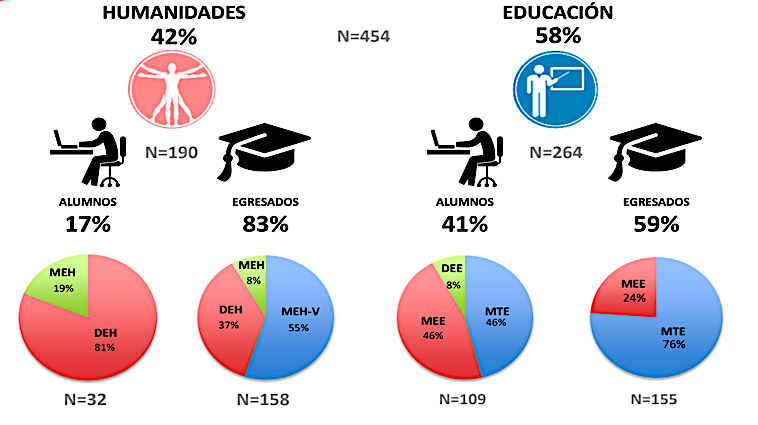
\includegraphics[width=0.8\textwidth]{Fig1.png}
 \caption{Estudiantes y egresados de posgrados en Humanidades y Educación.}
 \label{fig1}
 \source{del autor.}
\end{figure}

\subsection{Aplicación y análisis de datos}\label{sec-titulo}
La aplicación del cuestionario se hizo en línea y telefónica. Los datos se colectaron en una base de datos donde se realizaron análisis de las respuestas para llegar a asertos de incidencias \cite{stake_investigacion_2007} que fueron reducidos en categorías de análisis, para realizar sumas categóricas de asertos. Los datos se graficaron con Tableu y Vosviewer.

\section{Resultados}\label{sec-autores}

\subsection{Motivaciones}\label{sec-autores}
¿Cuál fue su principal motivación a la hora de decidir estudiar su posgrado?  Para ubicar el dato se cruzaron dos cuestionamientos: ¿qué programa estudia o estudió? y ¿cuál fue su principal motivación para estudiar su posgrado? Las motivaciones de los 361 participantes de maestría y de los 93 participantes relacionados con doctorado coincidieron en que su motivación principal era ampliar/profundizar sus conocimientos, seguido de mejorar oportunidades (\Cref{fig2}).
 
\begin{figure}[htbp]
 \hspace*{-1.3in}
 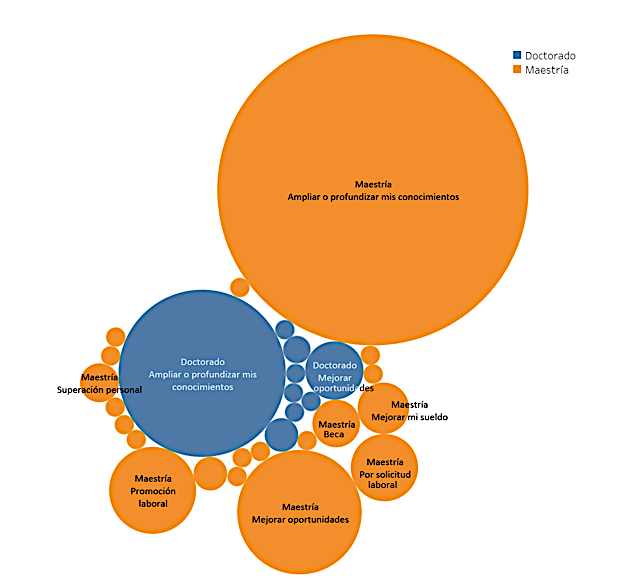
\includegraphics[width=1.22\textwidth]{Fig2.png}
 \caption{Motivación para estudiar su posgrado.}
 \label{fig2}
 \source{del autor.}
\end{figure}

\subsection{Conexión con necesidades}\label{sec-idioma}
En el rubro ¿cuándo considera que sus programas están desconectados con las necesidades actuales o futuras del entorno? Para ubicar el dato concreto se tomó la respuesta de quienes contestaron “No” en la pregunta ¿considera que los contenidos del plan de estudios, corresponden con las necesidades actuales o futuras del entorno? y la pregunta  ¿por qué? Los asertos de mayor frecuencia fueron poca investigación, poca innovación (que se vincula con la escasa práctica y formación metodológica), así como poco humanismo (vinculado con mucha teoría y el requerimiento de mejora de la calidad) (\Cref{fig3}).

\begin{figure}[htbp]
 \hspace*{-1.3in}
 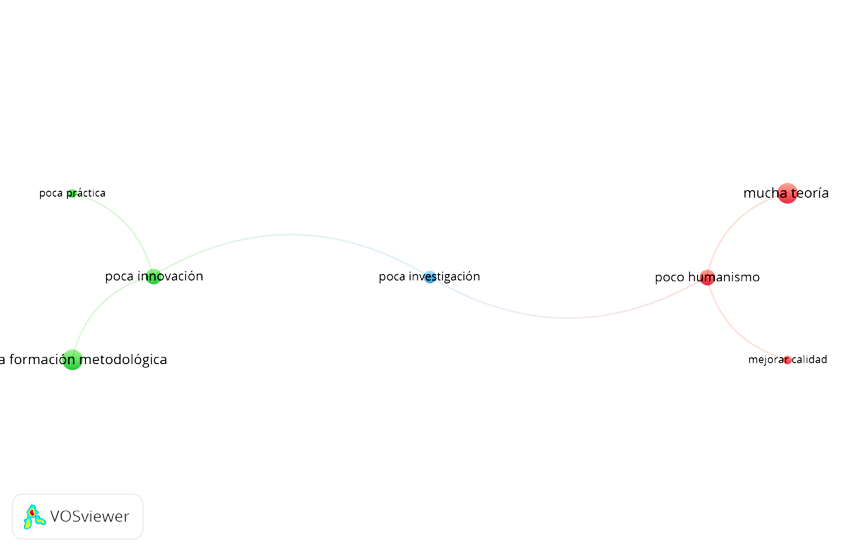
\includegraphics[width=1.22\textwidth]{Fig3.png}
 \caption{Asertos principales en la desconexión  de los programas.}
 \label{fig3}
 \source{del autor.}
\end{figure}

¿Qué competencia/habilidad/conocimiento no se incluye y considera que es importante incluir en sus programas? Para ubicar este dato se hizo análisis de la pregunta ¿qué programa estudia o estudió? Con los datos en las respuestas que otorgaron los participantes a la pregunta ¿qué competencia/habilidad/conocimiento no se incluye y considera que es importante incluir? Destaca en mayor incidencia la competencia de investigación, tanto para los estudiantes de maestría, como de doctorado. Seguido de competencias tecnológicas, idiomas y aplicación práctica, en participantes de maestría y de redacción de artículos, metodologías didácticas y habilidades blandas, en participantes de investigación (\Cref{fig4}).

\begin{figure}[htbp]
 \hspace*{-1.3in}
 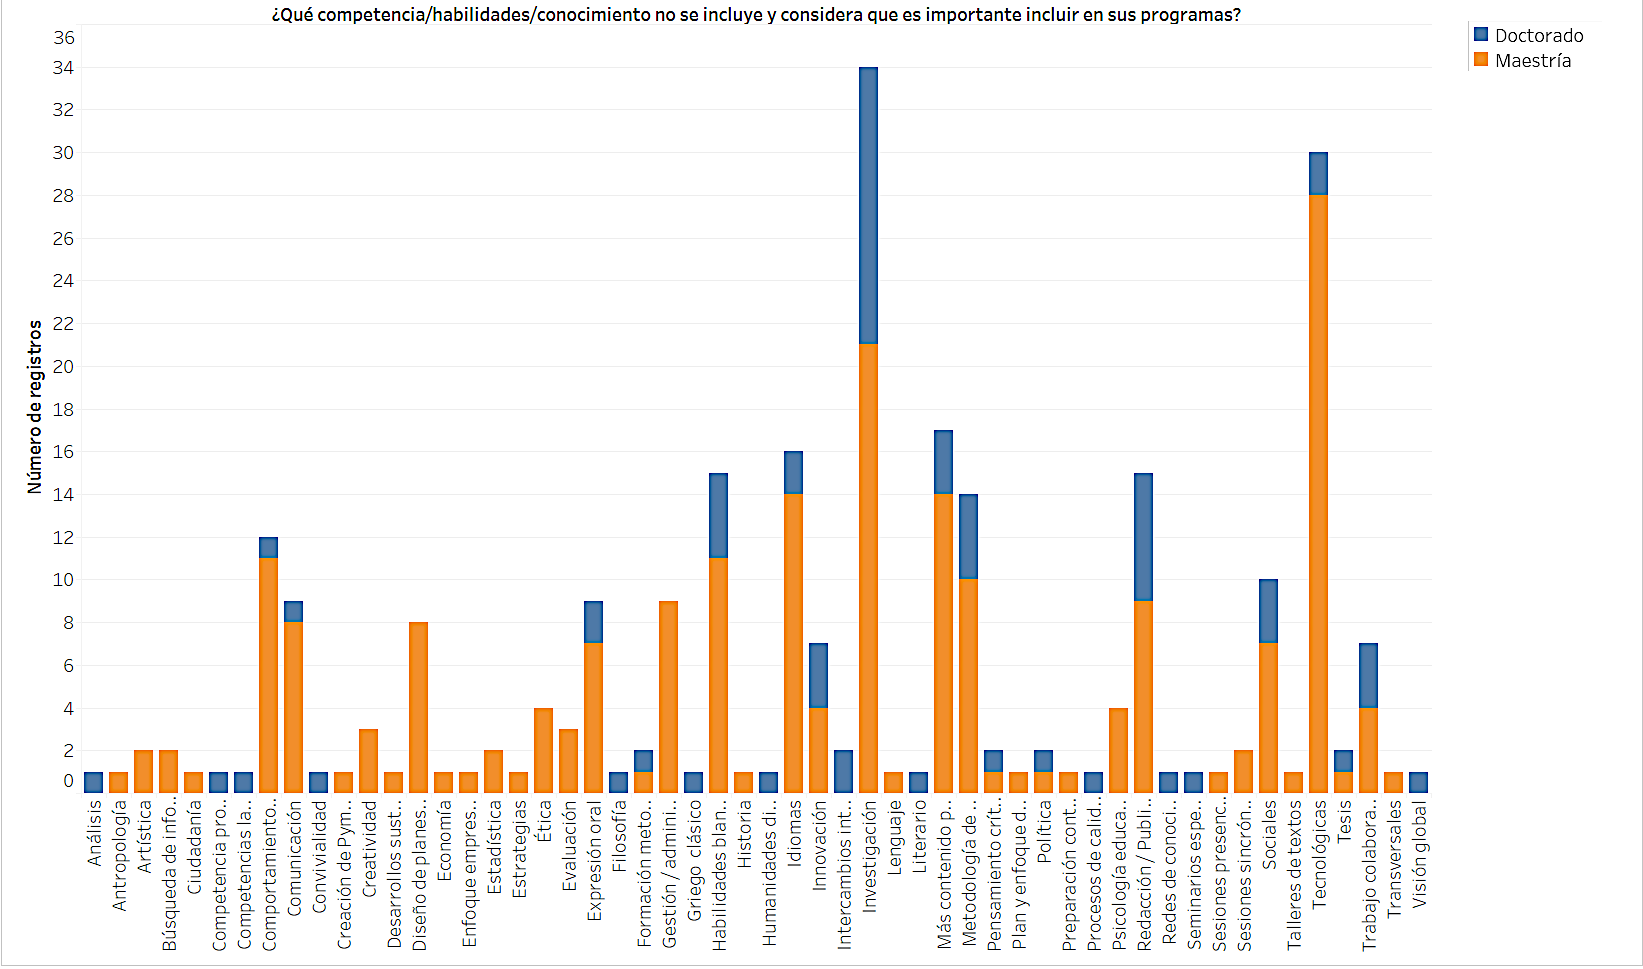
\includegraphics[width=1.22\textwidth]{Fig4.png}
 \caption{Competencia/habilidad/conocimiento para incluir en los programas formativos.}
 \label{fig4}
 \source{del autor.}
\end{figure}

¿En el ámbito laboral en qué proporción destina su tiempo a las actividades relacionadas con las áreas de Humanidades y Educación? se cruzó con la pregunta ¿en qué trabaja? Donde surgieron conceptos categóricos, con la interrogante ¿laboralmente, en qué proporción destina su tiempo a las siguientes actividades: investigación, docencia, consultoría, emprendimiento, gestión administrativa, medios / medios digitales o industria creativa? Los datos de mayor incidencia se dan en actividades relacionadas con la docencia en todas las actividades enunciadas, seguido de trabajo académico, gestión administrativa y consultoría (\Cref{fig5}).

\begin{figure}[htbp]
 \hspace*{-1.3in}
 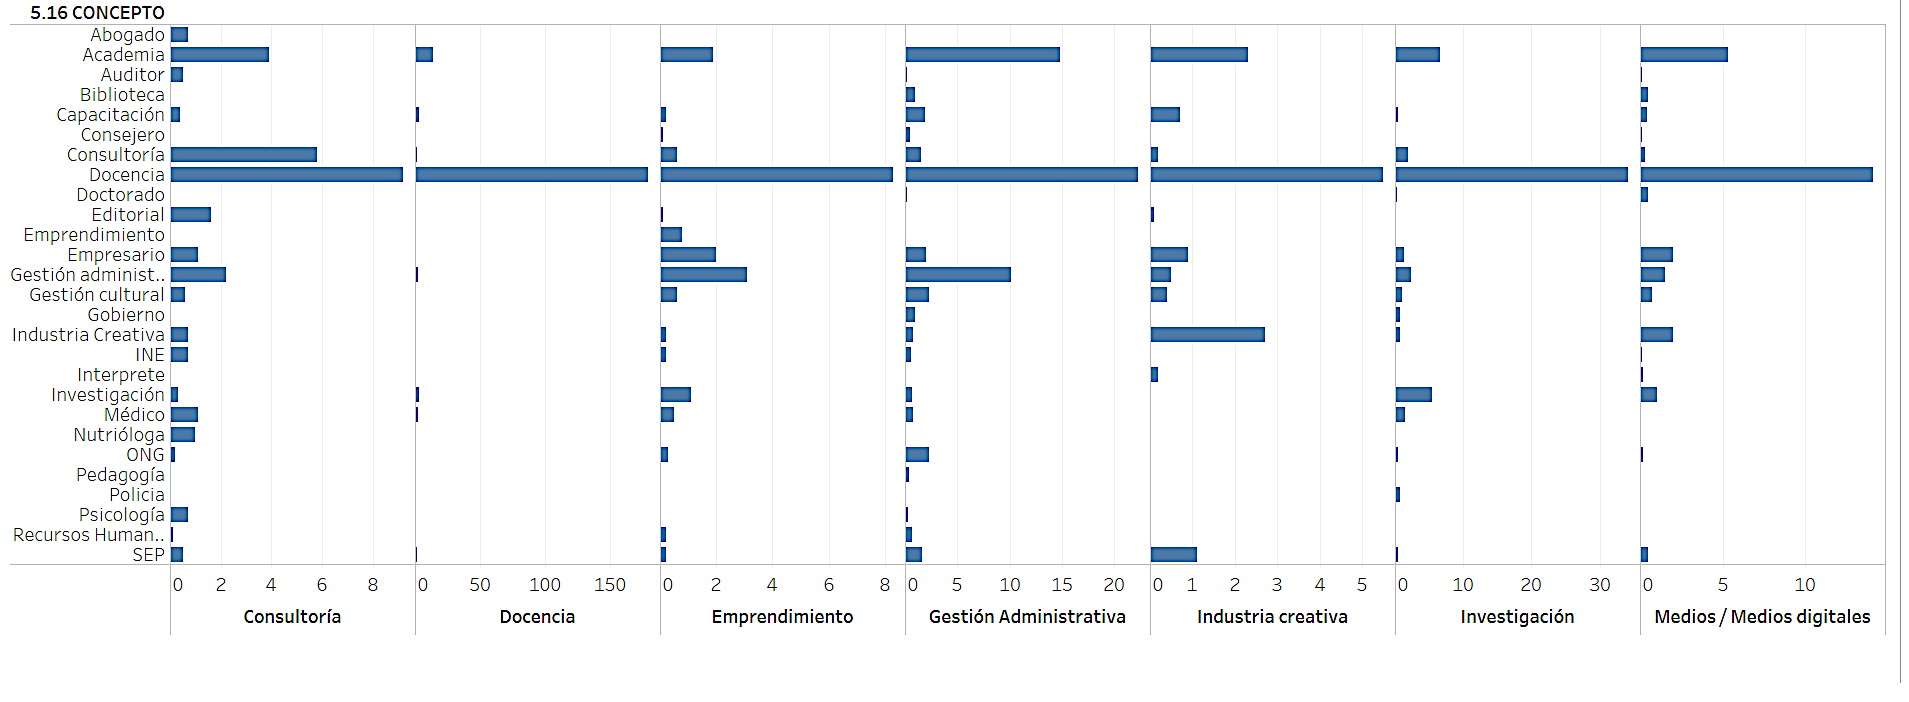
\includegraphics[width=1.22\textwidth]{Fig5.png}
 \caption{Actividades realizadas en los contextos laborales de los participantes.}
 \label{fig5}
 \source{del autor.}
\end{figure}

\subsection{Conocimientos para cambios}\label{sec-resumo}
¿Qué cambios y tendencias ve en su ámbito laboral? En el análisis de las respuestas se ubicaron asertos que fueron categorizados. Los resultados indican que son las TIC, la investigación y la innovación los cambios y tendencias que ubican de mayor incidencia y que además tienen una conexión en los co-términos; seguidos de capacitación, modelos educativos, modalidad educativa y virtualidad (que se relacionan con los co-términos de innovación y TIC) (\Cref{fig6}).

\begin{figure}[htbp]
 \centering
 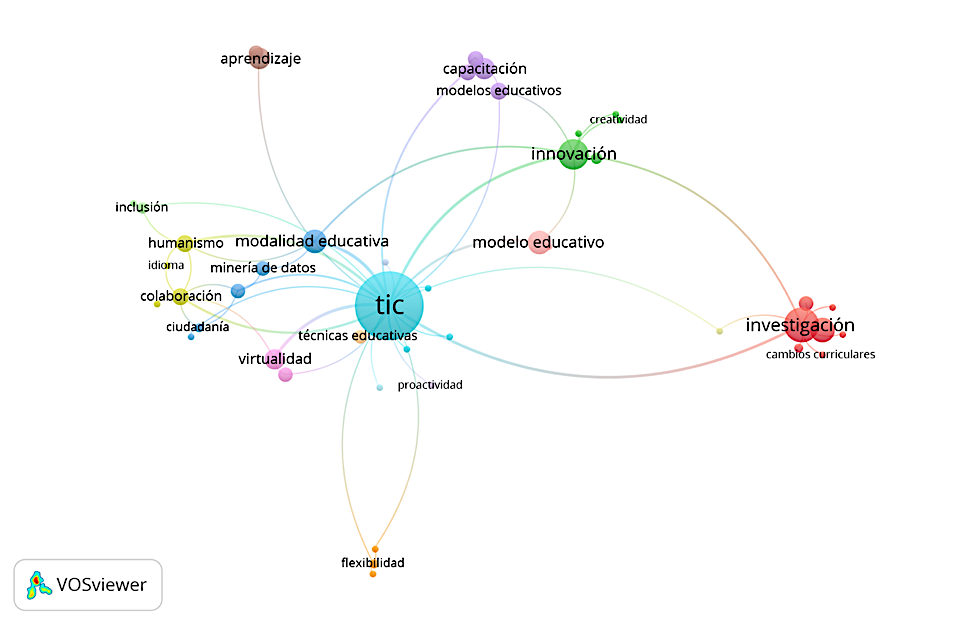
\includegraphics[width=\textwidth]{Fig6.png}
 \caption{Co-terminos relacionados de los cambios y tendencias
que se ubican en ámbitos laborales.}
 \label{fig6}
 \source{del autor.}
\end{figure}

¿Qué le demandan los cambios en su ámbito laboral? se analizaron las respuestas y se ubicaron sumas categóricas, destacando la actualización constante, la preparación, la capacitación y el uso de TIC, como las principales demandas que se reciben en sus ambientes de trabajo (\Cref{fig7}).

\begin{figure}[htbp]
 \centering
 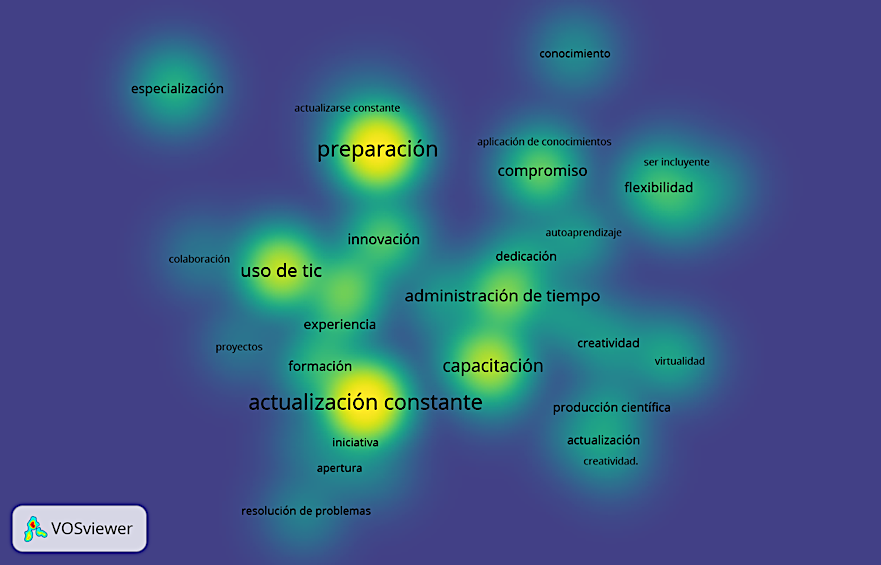
\includegraphics[width=\textwidth]{Fig7.png}
 \caption{Demandas en los ámbitos laborales.}
 \label{fig7}
 \source{del autor.}
\end{figure}

\section{Discusión}\label{sec-secoes}
Ubicar las motivaciones de los estudiantes de posgrado es importante para establecer un vínculo con los planes de estudio, las estrategias, los perfiles de egreso y los posibles ecosistemas digitales de los programas. La \Cref{fig2} evidencia, en mayor incidencia, que los estudiantes y egresados coinciden como principal motivación en la posibilidad de ampliar y profundizar los conocimientos. En estos esfuerzos, la autorregulación, a través de procesos de des-aprendizajes y cognición automátiva se relacionan con el valor que se encuentra en el conocimiento \cite{helfrich_how_2018}, así como aportar identidad y vida propia con ecosistemas digitales \cite{islas_ecosistemas_2017}. Los procesos de diseño y rediseños de programa tienen que contemplar evaluación diagnóstica para conocer los motores que llevaron a los participantes para estudiar un posgrado.

Establecer una conexión de los programas formativos con las necesidades actuales y futuras es un factor clave para desarrollar competencias que permitan aportar valor en diferentes ambientes. En la \Cref{fig3} destaca la poca investigación, innovación y humanismo, como elementos que ubican los participantes en sus programas desconectados con las necesidades; esto coincide con la \Cref{fig4} donde la investigación es la principal competencia que demandan los estudiantes y egresados de los posgrados. Estas demandas coinciden con las recomendaciones que dan \textcite{liang_how_2017} cuando enuncian que las bases de conocimiento juegan un papel cada vez más importante en muchas aplicaciones del mundo real, así como \textcite{dorsch_issue_2018} que sostiene que la ciencia relevante puede apoyar para aplicar la escolarización. En este sentido, se requieren análisis de los resultados de la investigación en ciencia, tecnología, humanidades e innovación y su impacto en el sector académico, social, productivo y gubernamental, para vincular los programas con las necesidades reales y futuras para contrarrestar la obsolescencia del conocimiento.

Una formación en posgrado requiere formar agentes de cambio para solucionar problemáticas del presente y adelantarse a situaciones futuras, con miras a aportar en el desarrollo sostenible. La \Cref{fig6} destaca los cambios y las tendencias en los contextos laborales, donde se ubican las TIC, la investigación y la innovación como elementos clave. De igual forma, la \Cref{fig7} en las sumas categóricas, destaca la actualización constante, la preparación, la capacitación y el uso de TIC, como las principales demandas que se reciben en sus ambientes de trabajo. En correspondencia con estos resultados, \textcite{milic_implementation_2017} mencionan la cuarta revolución tecnológica, donde se requería que los usuarios se adaptaran a las nuevas condiciones y nuevos conocimientos, asi como \textcite{picatoste_new_2018} que alertan sobre la innovación, como nuevo escenario que representa un desafío. Contemplar los conocimientos de la frontera del conocimiento será sustancial para integrar en los planes, y estrategias que busquen formar sujetos proactivos, más que reactivos ante la cotidianiedad de la vida diaria.


\section{Conclusiones}\label{sec-format-simple}
Apenas dos décadas han pasado del siglo XXI y mientras discutiamos la necesidad de adecuar los procesos formativos que contribuyeran a generar conocimientos y competencias útiles en las instituciones educativas, fuimos golpeados, una vez más, por el protagonismo de la aceleración de los procesos tecnológicos y un impacto de escala mundial llamada COVID 19.  

Estos hechos pusieron de manifiesto la importancia de defender la pluralización de voces y miradas y la necesidad de adecuar aceleradamente a las instituciones educativas a una nueva realidad;  un presente que pasó, en pocos meses, de una dinámica analógica a una digital, en todos los aspectos de la vida de las personas, obliga a todos los actores sociales que son parte de comunidades educativas, a unir miradas desde una perspectiva solidaria y propositiva, para buscar formas de generar y distribuir conocimientos y competencias para un futuro, que más que certezas presenta incertidumbre.

Se hace imprescindible que las instituciones educativas amplien la interacción multidisciplinaria, globalicen los conocimientos teórico prácticos de las novedosas estrategias didácticas, generalicen y profundicen el uso de las nuevas tecnologías y dejen de funcionar como compartimentos estanco para iniciar, de manera activa y constante, su vinculación con los diversos sectores de la sociedad. La necesidad de un análisis crítico del presente de las instituciones educativas y las propuestas formativas para sus estudiantes, permitirán dilucidar el nuevo rol y función que deberán cumplir.

Con estas reflexiones queda una invitación para seguir explorando datos que apoyen a contrarrestar conocimientos obsoletos donde se desarrollen capacidades científicas, tecnológicas y de innovación, como pilares para un desarrollo social sostenible. Trabajar solidariamente en programas que atiendan las demandas del contexto social y económico, para determinar contenidos interesantes de formación y donde se considere la vinculación con los sectores sociales, gubernamentales y empresariales, no solo académicos, como una acción estratégica y transversal para la formación de talento que aporte valor a la sociedad y al desarrollo sostenible.

\section{Agradecimientos}\label{sec-links}
Se agradece el apoyo de la decana (Inés Saénz) y de los directores de posgrado de la Escuela de Humanidades y Educación, para el diseño de los instrumentos. Así como la participación activa de estudiantes y egresados de posgrados, en especial a Maday Coronel por su apoyo con las Figuras.

\section{Agencia Financiadora}\label{sec-outras-estr}
Se agradece al CONACyT y al Instituto Politécnico Nacional, por el apoyo brindado para la realización del proyecto 312094 “Modelo de Continuidad Educativa para Situaciones de Crisis Sanitaria, a partir del Análisis de Buenas Prácticas, Lecciones y Retos en las IES Mexicanas durante la pandemia por COVID 19”,  a través del Convenio I12000/43/2019-MOD.ORD.18/2019-GENERAL-C-352/2020 con registro IPN SIP-2020-RE/02; del cual deriva este trabajo.

\printbibliography\label{sec-bib}

\end{document}
